\section{Theory}
\label{sec:theory}

% \subsection{Guarding the Polygon with One Point}
\subsection{Gradient Descent}

Let $\mathcal P$ be a polygon and $p(x, y) \in \mathcal P$ a guard. We are interested in computing the best direction for moving $p$ inside $\mathcal P$ such that the visibility area $Vis(p)$ increases. That is, exploring what would be a better position $p'$ to move $p$ to such that $p$ ``sees more'' of the polygon $\mathcal P$. 

We define $f(p)$ as the area seen by a guard $p$. Let $f'_r(p)$ be the local change in the area seen by guard $p$ around a reflex vertex $r$ seen by $p$ in $\mathcal P$, as given by the derivative of $f$. Given all reflex vertices $i$, the total (global) change in the area seen by $p$ can be thus summed up to $f'(p) = \sum_i f'_r(p)$. Figure \ref{fig:sumf} offers an example for this case for a polygon $\mathcal P$ and its reflex vertices $r_1$ and $r_2$. The polygon $\mathcal P$ is guarded by $p$, and its position is modified to $p'$ by a small change $\partial y$ in its $y$-coordinate. The visibility areas of $p$ are $f'_{r_1}$ and $f'_{r_2}$ around reflex vertices $r_1$ and $r_2$, respectively. In this way, the total change in the visibility area of $p$ is computed as $f'(p) = f'_{r_1}(p) + f'_{r_2}(p)$.

Thus, we consider $f(p)$ as the continuous objective function of The Art Gallery Problem. We can then use gradient descent as a method to optimise the objective function $f$. We will define below what the methodology of gradient descent is comprised of.

\begin{figure}[h!]
    \centering
    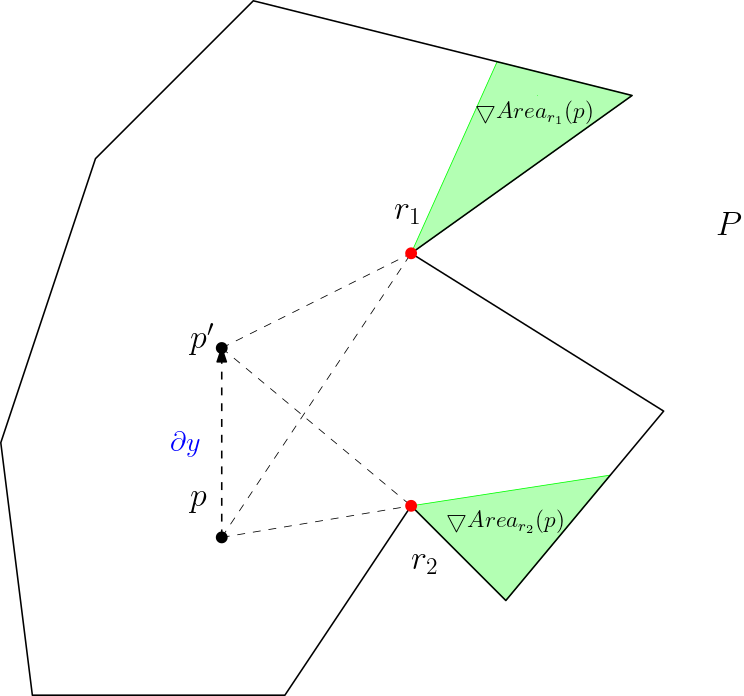
\includegraphics[width=0.4\textwidth]{theory/sumf.png}
    \caption{Global change in the area seen by $p$ when moved by $\partial y$ to a new position $p'$.}
    \label{fig:sumf}
\end{figure}


% Gradient descent is an iterative optimisation algorithm for finding the local optimum of a continuous differentiable function. The idea of gradient descent is to repeatedly move in the opposite direction of the gradient of the function at the current point. 
Let $\bigtriangledown f$ be the gradient of $f$. The gradient $\vec{\bigtriangledown f}$ then indicates the direction of the steepest descent for the objective function $f(p)$.
The learning rate (step size) $l$ is the size of the steps taken to reach the optimum. It is typically a small value, and it is evaluated and updated based on the behaviour of the optimisation function. 

After the gradient $\bigtriangledown f$ is computed, we can use it to calculate the new optimised position $p'$ of guard $p$: $$p'(x', y') = p'(x, y) + l\bigtriangledown f, l - \text{ learning rate}.$$

% High learning rates result in faster approaching towards the optimum, but risks overshooting it. Conversely, small learning rates are more precise, with the compromise of a longer computation and convergence time.

In later sections we will experiment with various learning rates. As such, we will explore how they influence the performance of our algorithm in relation to different test polygons. 

\newpage
\subsubsection{Computing the Gradient}

Given that $f$ is a function that describes the visibility area of a point $p(x, y)$, we first need to define how its gradient is computed. We will simplify the gradient computation without losing generality. As such, we will analyse the gradient by fixing one of the coordinates of $p$ and varying the other one. In this case, fixing the $x$-coordinate and varying the $y$-coordinate. The computation of the gradient remains the same regardless of the rotation applied to the plane.


We will use the notation $\frac{\partial f}{\partial y}$ to denote the change in the visibility area $f(p)$ when the $y$-coordinate is modified by a small amount $\partial y \rightarrow 0$. Analogously, we will use $\frac{\partial f}{\partial x}$ to denote the small change in the $x$-coordinate of $p$. In this way, we define 

\begin{equation}
    \bigtriangledown f = (\frac{\partial f}{\partial x}, \frac{\partial f}{\partial y})^\intercal \label{eq:gradient}
\end{equation}

to be the gradient of $f$ given that $\mathcal P$ is guarded by a point $p(x, y)$. 

We will now create a canonical geometrical construction that allows us to further define and compute $\vec{\bigtriangledown f}$. In this case, we consider the normalised length of the gradient as $||\vec{\bigtriangledown f}||~=~1$. This canonical construction is displayed in Figure \ref{fig:gradient}. 
% We will then generalise this case to multiple reflex vertices and guards.

\begin{figure}[h!]
    \centering
    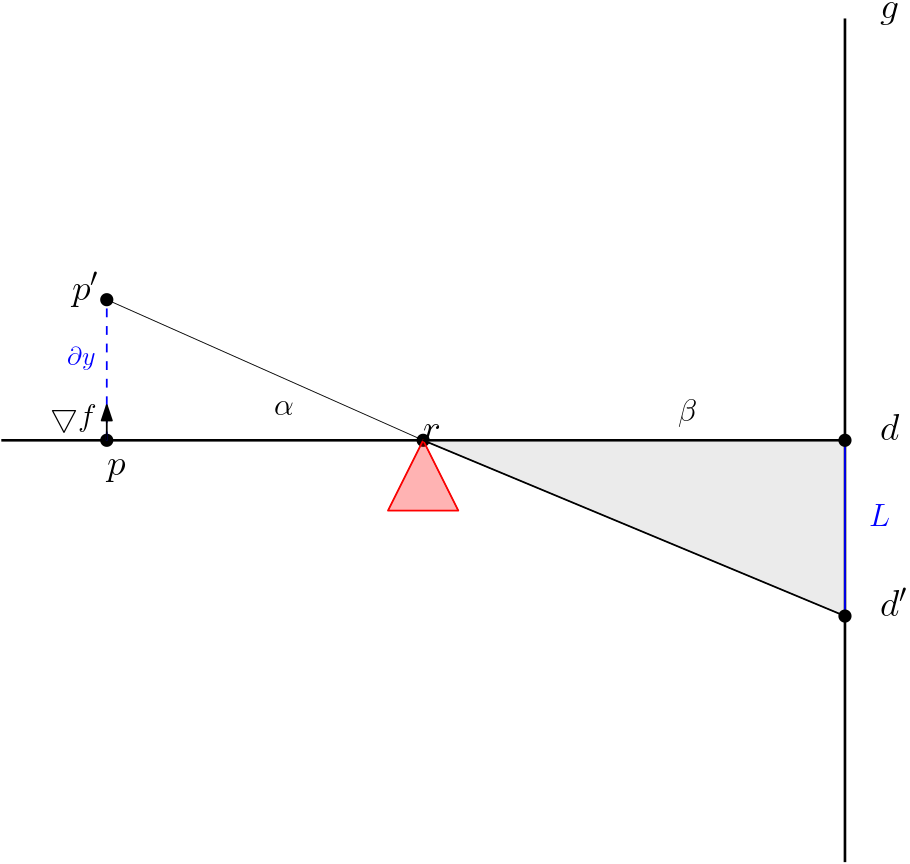
\includegraphics[width = 0.6\textwidth]{theory/gradient2.png}
    \caption{Canonical gradient construction and for when the position of $p$ is varied by a small amount $\partial y$ around reflex vertex $r$ to the new position $p'$.}
    \label{fig:gradient}
\end{figure}

Let $g$ be a boundary line segment of $\mathcal P$, $r$ a reflex vertex inside $\mathcal P$ and $p$ a guard whose optimal position we are interested in. The reflex vertex $r$ is seen by $p$. Let $\overline{pr} = \alpha$ be known. Additionally, let $d$ be the maximum point of visibility that $p$ can see behind $r$ on the line $g$. Let the distance between $r$ and $d$ be considered as $|\overline{rd}| = \beta$ known. 
% That is, the direction of the greatest increase of $f$. 

% We consider the case where there is only a positive change in the $y$ position of $p$. The case with a negative coordinate change would be analogous.


Let $\partial y$ be an extremely small change in the $y$-coordinate of $p$. Let $p'$ be the new position of $p$ given the change $\partial y$. The point $p'$ can see then up to a new maximum point $d'$ around $r$ on $g$. Let thus the distance between $d$ and $d'$ be $|\overline{dd'}| = L$. As such, $\triangle rdd'$ denotes the increase in the visibility area of $p$ when it moves to position $p'$. That is, the first derivative $f'(p)$ of $f$ will represent the change in the visibility area of $p$:

\begin{equation}
    \text{Area}_{\triangle rdd'} = f'_r(p). \label{eq:derivative}
\end{equation}

% Let $a''$ be the projection of $p'$ on $p''r$, and $a$ the projection of $a''$ on the line $pr$ such that the distance from $a$ to $r$ is $|\overline{ar}| = \alpha$. Take the distance between $p$ and $p'$ to be $x$. Since $a''$ is the projection of $p'$ on $pr$, then $|\overline{pp'}| = |\overline{aa''}| = x$.





% \subsection{Canonical Case}
% Consider the geometrical construction in Figure \ref{fig:gradient}. The construction was created for ease of computation, and the general case can be translated and rotated to this case.

% In this canonical case we will consider the situation where the gradient is normalised as $||\bigtriangledown f|| = 1$. 

We are now interested in computing how the area seen by guard $p$ increases given the change $\partial y$ in the position of $p$. The distances $||\overline{pr}|| = \alpha$ and $||\overline{rd}|| = \beta$ are known. As such, we aim at expressing the gradient $\bigtriangledown f_r$ for point $p$ and reflex vertex $r \in Vis(p)$ using $\alpha$ and $\beta$. Since $\bigtriangledown f_r$ depends on the change in the coordinates of $p$, computing it is tightly connected to the change in the area of triangle $\triangle rdd'$. We will proceed to calculate the area of $\triangle rdd'$ below.
% We are now interested in computing the distances $|\overline{df}|, |\overline{aa'}|, |\overline{pp''}|, L$ such that we can compute the increase in the area seen by $p$ and thus the gradient $\bigtriangledown f$. The two triangle areas that need to be computed in order to do so are $A_{\triangle rdd'}$ and $A_{\triangle rdd''}$.

Given that triangles $\triangle rpp'$ and $\triangle rdd'$ are square triangles, their areas can be calculated as:

\begin{align}
    \text{Area}_{\triangle rpp'} &= \frac{\alpha \partial y}{2}, \label{eq:rpp}\\
    \text{Area}_{\triangle rdd'} &= \frac{\beta L}{2}. \label{eq:rdd}   
\end{align}


Given that $\overline{pp'}$ is parallel to $g$, we can use Thales's Theorem in triangles $\triangle rpp'$ and $\triangle rdd'$ to compute the length $L$: 

\begin{align}
    \frac{||\overline{pp'}||}{||\overline{dd'}||} &= \frac \alpha \beta \\
    \frac{\partial y}{L} &= \frac \alpha \beta  \label{eq:dxL} \\
    L &= \frac{\beta \partial y}{\alpha}. \label{eq:L}
\end{align}


% we can compute the length $L$: $$\frac{\text{Area}_{\triangle rdd'}}{\text{Area}_{\triangle rpp'}} = \frac{\frac{\beta L}{2}}{\frac{\alpha \partial x}{2}} = \frac{\beta L}{\alpha \partial x} \Rightarrow L = \frac{\partial x \beta}{\alpha}.$$

We are now interested in how areas $\text{Area}_{\triangle rpp'}$ and $\text{Area}_{\triangle rdd'}$ change depending on how $\alpha$ and $\beta$. That is, $\frac{\text{Area}_{\triangle rdd'}}{\text{Area}_{\triangle rpp'}}$ as a function of $\alpha$ and $\beta$: 

\begin{align}
    \frac{\text{Area}_{\triangle rpp'}}{\text{Area}_{\triangle rdd'}} \overset{(\ref{eq:rpp}), (\ref{eq:rdd})}{=} &\frac{\frac{\alpha \partial y}{2}}{\frac{\beta L}{2}} \\
    = &\frac{\alpha \partial y}{\beta L} \\
    \overset{(\ref{eq:dxL})}{=} &\frac{\alpha \alpha}{\beta \beta} \\
    \frac{\text{Area}_{\triangle rpp'}}{\text{Area}_{\triangle rdd'}} = &{(\frac \alpha \beta)}^2 \label{eq:rddrpp}
\end{align}

We can now express the area of $\triangle rdd'$ as only dependent on $\alpha, \beta$, the small position change $\partial y$ and the already known area of $\triangle rpp'$:

\begin{align}
    \text{Area}_{\triangle rdd'} \overset{(\ref{eq:rddrpp})}{=} &{(\frac \beta \alpha)}^2 \text{Area}_{\triangle rpp'} \\
    \overset{(\ref{eq:rpp})}{=} &{(\frac \beta \alpha)}^2 \frac{\alpha \partial y}{2} \\
    \text{Area}_{\triangle rdd'} = &\frac{\beta^2 \partial y}{2\alpha}. \label{eq:ardd}
\end{align}
% \end{align*}
% $$\frac{\partial f}{\partial x} = \frac{\text{Area}_{\triangle rdd'}}{\partial x}$$

Analogously, we can compute the change in the $y$-coordinate by rotating the plane with $90^\circ$ and follow the same steps. This procedure will result in

\begin{equation}
    \text{Area}_{\triangle rdd'} = \frac{\beta^2 \partial y}{2\alpha}. \label{eq:ardd2}
\end{equation}

We can now compute the change in the visibility area of $p$ ($\text{Area}_{\triangle rdd'}$) given the movement $\partial y$ around reflex vertex $r$. Since the $x$-coordinate of $p$ is fixed, $\partial x = 0$. So, we can compute the gradient $\bigtriangledown f_r$ for a point $p$ and one of the reflex vertices $r$ seen by $p$ as

\begin{align*}
    \bigtriangledown f_r \overset{(\ref{eq:gradient})}{=} &(\frac{\partial f}{\partial x}, \frac{\partial f}{\partial y})^\intercal \\
    \overset{(\ref{eq:derivative})}{=} &(0, \frac{\text{Area}_{\triangle rdd'}}{\partial y} + \partial y)^\intercal \\
    \bigtriangledown f_r \overset{(\ref{eq:ardd}), (\ref{eq:ardd2})}{=} &(0, \frac{\beta^2}{2\alpha} + 0)^\intercal \\
    \bigtriangledown f_r = &(0, \frac{\beta^2}{2\alpha})^\intercal.
\end{align*}

Analogously, when only the $x$-coordinate of $p$ is modified around a reflex vertex $r \in Vis(p)$, the gradient becomes $$\bigtriangledown f_r = (\frac{\beta^2}{2\alpha}, 0)^\intercal.$$

Therefore, for all the reflex vertices $r$ guard $p$ can see, the total gradient $\bigtriangledown f$ becomes the sum of all the partial gradients $\bigtriangledown f_r$ as $$\bigtriangledown f = \sum_r \bigtriangledown f_r, \forall r \text{ reflex vertex } \in Vis(p).$$

\subsubsection{Computing the New Guard's Position}
We can now use the coordinates of the gradient $\bigtriangledown f$ to compute the movement direction of the guard $p$ given all the reflex vertices from $\mathcal P$ seen by $p$. In order to do so, we will use the construction depicted in Figure \ref{fig:vperp}. 

\begin{figure}[h!]
    \centering
    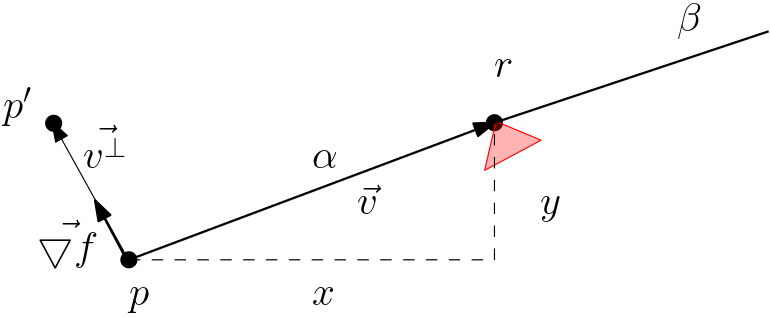
\includegraphics[width = 0.5\textwidth]{theory/v_perp.png}
    \caption{Computing the new position $p'$ of guard $p$ around reflex vertex $r$ based on the gradient $\bigtriangledown f$.}
    \label{fig:vperp}
\end{figure}

Let $\vec v$ be the vector corresponding to the direction of movement from guard $p$ to a reflex vertex $r$, such that $\vec{v} = (r - p) = (x, y)^\intercal$, with norm $||v|| = \alpha$. So, $||\frac{\vec v}{\alpha}|| = 1$.

Let $\vec{v}^\perp  = (p' - p)$ be the vector corresponding to the direction of movement from guard $p$ to its new position $p'$. Vector $\vec v^\perp$ is orthogonal to $\vec{v}$, in the same direction as $\vec{\bigtriangledown f}$, such that $||\vec{v}|| = ||\vec{v}^\perp|| = \alpha$. We will use the coordinates of $v^\perp$ to compute the coordinates of $\bigtriangledown f$ and thus the direction in which $p$ needs to move.

The coordinates of $\vec v^\perp$ can then be computed using the construction from Figure \ref{fig:vsquare}. Since $\vec v^\perp \perp \vec v$, and $p$ and $r$ are on the right-hand side of $\vec v^\perp$, the coordinates of $\vec v^\perp$ will be rotated by $-90^\circ$ so that $\vec v^\perp = (-y, x)^\intercal$. Analogously for the case when $p$ and $r$ are rotated by $180^\circ$ to the left-hand side of $\vec v^\perp$, the coordinates of $\vec v^\perp$ will be rotated by $90^\circ$ to $\vec v^\perp = (-x, y)^\intercal$.

\begin{figure}[h!]
    \centering
    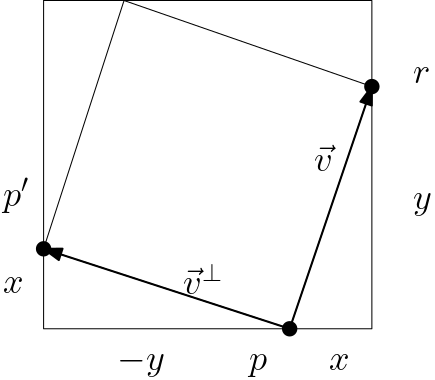
\includegraphics[width = 0.35\textwidth]{theory/v_square.png}
    \caption{Computing the coordinates of $\vec v^\perp$ given the guard $p$ and the reflex vertex $r(x, y)$.}
    \label{fig:vsquare}
\end{figure}

We know that the norm of the gradient is $||\vec{\bigtriangledown f}|| = \frac{\beta^2}{2\alpha}$. Since $\vec{\bigtriangledown f}$ has the same direction as $\vec v^\perp$, we wish to normalise it from the norm of $\vec v^\perp$ with $\frac 1 \alpha$. Therefore, the gradient for guard $p$ and one reflex vertex $r \in Vis(p)$ can be computed as $$\vec{\bigtriangledown f} = \vec v^\perp \frac{\beta^2}{2\alpha} \frac 1 \alpha.$$

As mentioned before, the total gradient for guard $p$ and all the reflex vertices $r$ the guard can see is $$\vec{\bigtriangledown f} = \sum_r \vec{\bigtriangledown f_r}, \forall r \text{ reflex vertex } \in \mathcal P.$$

The new position $p'$ of guard $p$ based on all the reflex vertices it can see is: 
\begin{equation}
    p'(x', y') = p'(x, y) + l\bigtriangledown f, l - \text{ learning rate}.
    \label{eq:l}
\end{equation}




% Given that $pp''$ is parallel to $g$, we can use the Intercept Theorem to compute the lengths of the segments as follows:

% \begin{itemize}
%     \item in $\triangle raa'$, $\triangle rpp'$, with $aa' || pp'$: $$\frac{|\overline{pp'}|}{|\overline{dd'}|} = \frac{|\overline{pr}|}{|\overline{rd}|} \iff \frac{x}{|\overline{dd'}|} = \frac{1}{\beta} \Rightarrow |\overline{dd'}| = x\beta$$
    
%     $$\frac{|\overline{aa'}|}{|\overline{pp'}|} = \frac{\alpha}{1} = \frac{|\overline{aa'}|}{x} \Rightarrow |\overline{aa'}| = x\alpha$$

%     \item in $\triangle rpp''$, $\triangle raa''$, with $pp'' || aa''$: $$\frac{|\overline{aa''}|}{pp''} = \frac{|\overline{ar}|}{|\overline{pr}|} \iff \frac{x}{|\overline{pp''}|} = \frac{\alpha}{1} \Rightarrow |\overline{pp''}| = \frac{x}{\alpha}$$
    
%     \item in $\triangle rpp''$, $\triangle rdd''$, with $pp'' || dd''$: $$\frac{|\overline{pp''}|}{|\overline{dd''}|} = \frac{|\overline{pr}|}{|\overline{rd}|} \iff \frac{\frac{x}{\alpha}}{L} = \frac{1}{\beta} \Rightarrow L = \frac{x\beta}{\alpha}$$
% \end{itemize}

% Now the area of the square triangle $\triangle rdd''$ corresponding to the gradient $\bigtriangledown f$ can be computed as: $$\bigtriangledown f = \frac{|\overline{rd}||\overline{de}|}{2} = \frac{\beta L}{2} = \frac{\beta \frac{x\beta}{\alpha}}{2} = \frac{\beta^2x}{2\alpha}, ||x|| = 1$$


% \subsection{General Case}


% - we will only look at one coordinate (vary $y$), since varying $x$ is symmetrical, but rotated $90^\circ$

% - we will first look at a canonical situation $||\bigtriangledown f|| = 1, \alpha = \beta = 1$

% Let:

% - $f(p)$ - area seen by guard $p$

% - $f'_i(p)$ - the change in the area seen locally by guard $p$, as given by its derivative

% - $f'(p) = \sum_i f'_i(p)$ - the change in the area seen globally by guard $p$

% - $\bigtriangledown f = (\frac{\partial f}{\partial x}, \frac{\partial f}{\partial y})$ - the direction of the greatest increase of $f$

% - $r$ - reflex vertex

% - $p$ - guard whose position needs to be optimised

% - $|\overline{pr}| = 1$

% - $p', p''$ - the new positions of the guard where the $y$-coord is varied

    % - $|\overline{pp'}| = |\overline{aa''}| = x$

% - $\overline{ar} = \alpha, a \in \overline{pr}$ - additional guard construction

% - $\triangle rde$ - area seen by $p$

    % - $\triangle rdf$ - area seen by $p'$

% - $|\overline{rd}| = \beta$ - distance between reflex vertex and polygon boundary

% - $|\overline{de}| = L$

% Using the Intercept Theorem:

% - in $\triangle ra'a$, $\triangle rp'p$: $\frac{|\overline{pp'}|}{|\overline{df}|} = \frac{|\overline{pr}|}{|\overline{rd}|} = \frac{x}{|\overline{df}|} = \frac{1}{\beta} \Rightarrow |\overline{df}| = x\beta$

% - in $\triangle pp'r$, $\triangle aa'r$: $\frac{|\overline{aa'}|}{|\overline{pp'}|} = \frac{\alpha}{1} = \frac{|\overline{aa'}|}{x} \Rightarrow |\overline{aa'}| = x\alpha$

% - in $\triangle pp''r$, $\triangle aa''r$: $\frac{|\overline{aa''}|}{pp''} = \frac{|\overline{ar}|}{|\overline{pr}|} = \frac{x}{|\overline{pp''}|} = \frac{\alpha}{1} \Rightarrow |\overline{pp''}| = \frac{x}{\alpha}$

% - in $\triangle pp''r$, $\triangle rde$: $\frac{|\overline{pp''}|}{|\overline{de}|} = \frac{|\overline{pr}|}{|\overline{rd}|} = \frac{\frac{x}{\alpha}}{L} = \frac{1}{\beta} \Rightarrow L = \frac{x\beta}{\alpha}$

% Computing the area of the square triangle $\triangle rde$:

% - $A = \frac{|\overline{rd}||\overline{de}|}{2} = \frac{\beta L}{2} = \frac{\beta \frac{x\beta}{\alpha}}{2} = \frac{\beta^2x}{2\alpha}$